%\documentclass[../Manuscrit.tex]{subfiles}
\documentclass[../eBook.tex]{subfiles}

\begin{document}
    \paragraph{}En suivant la lecture des Registres de l'Etat civil de la commune de Sermaise, dont le plus ancien, nous l'avons dit, est de 1675, on peut établir la liste de tous les Instituteurs qui ont exercé dans la commune depuis plus de deux siècles.

    \phantomsection
    \addchapterline{Avant 1789}
    \subsection*{Avant 1789}
      \paragraph{}\textit{Leloup} François (1675 - 1680) ; \textit{Perrolat} Jacques (1680 - 1686) ; \textit{Lamiral} François (1686 - 1689) ; \textit{Hérué} Pierre (1689 - 1695) ; \textit{Legendre} Barthélemy (1695 - 1698) ; \textit{Noustre} Louis (1698 - 1699) ; \textit{Lerebours} (Louis) 1699 - 1700 : À la fin de l'année 1700, ce maître passa prêtre-vicaire à Sermaise ; \textit{de Beauvoisins} Charles (1700 - 1709) ; \textit{Boizard} Jacques (1709 - 1713) ; \textit{Savouré} Denys (1713 - 1718) ; \textit{Isambert} Michel (1718 - 1727) ; \textit{Guischard} François (1727 - 1730) ; \textit{Leblanc} Pierre (1730 - 1739).
      \paragraph{}Ces maîtres d'école qui sont au nombre de treize ont occupé le poste de Sermaise pendant 64 ans, ce qui fait une moyenne de près de cinq années chacun. Il est impossible de connaître les locaux qui leur ont servi d'école. Sans doute ils étaient chantres car on les rencontre témoins de tous les actes d'inhumation et souvent avec le bedeau. Il y a lieu de croire aussi qu'ils étaient originaires de Sermaise, la plupart des actes de l'église étant signés par eux avant et après leurs fonctions de maîtres d'école. Leurs signatures sont très lisibles et généralement en belle bâtarde.
      \paragraph{}Les maîtres qui ont succédé à ceux que l'on vient de citer ont tenu classe d'abord dans une maisonnette qui est encore debout mais non habitée et appartenant à M. Boudon. La pièce où se faisait l'école a 5 \textit{m} 50 de long, 3 \textit{m} 50 de large et 3 \textit{m} de haut ; le jour n'y pénétrait que par une seule croisée, et le maître n'avait qu'une pièce très exiguë et un grenier. L'immeuble est situé près de l'église sur la place publique et les anciens collègues qui en ont fait leur résidence sont :
      \begin{itemize}[noitemsep]
        \setlength{\baselineskip}{16pt}
        \item[] \textit{Gautier} Jean (1739 - 1793) -- c'est lui qui en 1793 rédigea le premier acte signé par un officier de l'état civil, et à partir de cette époque la mairie a été tenue par les Instituteurs qui ont exercé à Sermaise ;
        \item[] \textit{Gautier} Denis Bernard fils du précédent (1793 - 1796) ;
        \item[] \textit{Faguet} (1796 - 1797).
      \end{itemize}

      \phantomsection
      \addsectionline{Règles et moyens employés par le M Gautier père pour encourager les enfants à bien apprendre}
      \subsubsection*{Règles et moyens employés par le M Gautier père pour encourager les enfants à bien apprendre}
        \begin{quote}
          \begin{sloppypar}
            \og \textit{En premier lieu, au commencement, le Maistre d'école baillera à chacun enfant trois privilèges chacun desquels empêchera d'estre battu sinon que la faute fust trop grande. Le Maistre placera les enfants sur plusieurs bancs suivant capacitez et sur chaque banc fera asçoir dix enfants ou plus (si tant y en a) d'une même capacitez, le premier desquels sera celuy qui dira le mieux la leçon ; le second après, etc.
            \paragraph{}Le premier de chacun banc sera assis au haut bout, aura un nom honorable et sera exempt d'estre battu tant qu'il sera le premier s'il ne commet quelque grande faute. Celuy qui de chacun banc sera le dernier sera appelé le dernier ou aura quelqu'autre nom suivant la prudence du maistre. Le Maistre baillera une heure aux enfants pour venir à l'escole, laquelle heure passée celui qui viendra devant son prochain compagnon gagnera sa place : les enfants estant arrivez, le Maistre les fera prier Dieu puis à chacun d'eux leur baillera une mesme leçon.
            \paragraph{}Le Maistre commencera au premier banc et fera venir devant soi tous les enfants de ce banc et commencera au premier auquel en sa présence du second il fera dire sa leçon. Si le premier manque à sa leçon trois fois et que le second le corrige les trois fois il aura sa place et le second sera le premier et cette correction que le second aura luy servira de leçon, puis le Maistre fera dire la mesme leçon au troisième en la présence du quatrième, que si le troisième fait des fautes et que le quatrième les corrige trois fois il aura sa place et ainsi des autres ce qui sera observé en tous les bancs. Les enfants ayant tous dit leurs leçons le Maistre les fera agenouiller et au premier fera dire Benedicite, etc. et puis les fera déjeuner.
            \paragraph{}Ce fait le Maistre fera répéter aux enfants leur leçon, fera venir devant luy les enfants du premier banc et commencera au dernier en la présence de celuy qui le suit auxquels deux il fera répéter leur leçon, ce fait le dernier montrera à celuy qui est proche devant luy trois mots difficiles si des trois il en ignore un seulement il ne perdra pas sa place mais s'il manque deux ou trois fois et que le dernier le corrige il aura sa place. Ce fait le Maistre fera répéter au suivant en présence de celuy qui a gagné la place lequel taschera encore de gaigner sa place et lui fera trois questions desquelles s'il en corrige deux ou trois il aura encore sa place et ainsi le maistre continuera à faire répéter et questionner jusques au premier pour avoir sa place duquel il faudra qu'il aye manqué les trois fois et que celuy qui le précède le corrige et ainsi de banc en banc et ce par chacun tous la matinée et l'après-midy. Le Maistre d'Escolle ne chastiera les enfants en cholère ne les outragera, ainsi les gouvernera par prudence et fera en sorte que nul ne s'en retourne qu'il n'ait appris quelque chose de nouveau chaque jour}. \fg{}
          \end{sloppypar}
        \end{quote}
        \paragraph{}Les enfants étaient reçus à l'école quand ils pouvaient bien prononcer : \og \textit{Credo in Deum Patrem, credo in Jesum christum, credo in spiritum sanctum}.\fg{}

    \phantomsection
    \addchapterline{Après la Révolution}
    \subsection*{Après la Révolution}
      \paragraph{}\textit{Chevallier} (Félix) a été instituteur à Sermaise de 1797 à 1828. Il avait passé quelques années au séminaire de Versailles, mais se sentant une vocation pour l'enseignement de la jeunesse il quitta l'habit de prêtre et vint tenir l'école de Sermaise. Par son instruction assez développée et par sa bonne tenue il s'attira l'attention des familles et son école était fréquentée non seulement par les élèves de Sermaise mais aussi par ceux des hameaux voisins dépendant des communes de Roinville, Villeconin \& S\up{t}-Chéron. Outre ses fonctions d'instituteur et de chantre, il a exercé aussi celles de receveur municipal \& d'adjoint au Maire. Avec la rétribution scolaire qui était de 0\up{\uppercase{F}}75 par mois il recevait un pain mensuel par élève, de 1 \textit{kilogr} 1/2, et à cause des bons services qu'il rendait aux habitants, ils lui fournissaient le vin \& le cidre nécessaire à sa consommation.
      \paragraph{}Gautier père et fils, dont il a été parlé plus haut et Chevallier étaient propriétaires de la maison où ils tenaient classe, ils recevaient de la part de la commune la somme de 30 francs à titre d'indemnité de logement.
      \paragraph{}Depuis 1793 jusqu'à 1807, le greffe de la mairie donna un traitement de 18 francs et le montage de l'horloge un traitement de 25 francs. En 1825, l'instituteur Chevallier avait en dehors de sa rétribution scolaire un traitement de 40 \textit{fr} pour la Mairie, de 25 francs pour l'horloge communale, un supplément de 50 francs, une indemnité de logement de 30 francs, soit 145 francs d'allocations diverses.
      \paragraph{}Aucune liste de gratuité n'était dressée, mais malgré cela le curé qui visitait souvent l'école et la couvrait d'une grande protection désignait les enfants qui devraient recevoir l'instruction gratuite.
      \paragraph{}\textit{Hardy} Félix a exercé de 1828 à 1848. Cet instituteur fit l'école dans une maison qui était sa propriété et qui est encore occupée par sa famille. Elle offrait une salle de classe plus convenable sous tous les rapports que celle qui servit pendant 89 ans et dont on a parlé plus haut.
      \paragraph{}En 1831, la commune paya à M. Hardy une indemnité de logement de 80 francs. En 1833, le 22 septembre, le conseil municipal de la commune de Sermaise, en vertu de la loi du 28 juin de la même année, se réunit et prit les dispositions suivantes :
      \paragraph{}\og \textit{Le Conseil municipal est d'avis que l'instruction dans la commune de Sermaise soit portée instruction primaire élémentaire. Le taux de la rétribution est de 0\up{\uppercase{F}}75, 1 \textit{fr}, 1 \textit{fr} 25, 1 \textit{fr} 50, 1 \textit{fr} 75. Le traitement fixe de l'Instituteur est de 200 francs.
      \paragraph{}Le Conseil est d'avis qu'il soit porté un nombre de 10 élèves gratuits à l'instruction primaire élémentaire.} \fg{}
      \paragraph{}L'année suivante le nombre de gratuits est porté à 12. En 1836, la rétribution mensuelle est fixée à 1 \textit{fr} pour la première classe, 1 \textit{fr} 50 pour la seconde et 1 \textit{fr} 75 pour la 3\up{e}.
      \paragraph{}Les enfants qui fréquentaient alors l'école étaient au nombre de 35 l'été et de 55 l'hiver. Ceux en âge de la fréquenter étaient de 70.
      \paragraph{}Le 11 mai de cette même année la commune fit l'acquisition moyennant la somme de 4200 francs d'une maison appartenant à M. Veillard pour y installer l'école communale. Les dimensions de la salle de classe étaient : 8 mètres de long, 5 mètres de large, 3 mètres de haut. Le logement de l'Instituteur se composait d'une chambre froide \& d'une chambre à feu.
      \paragraph{}En 1842, le taux de la rétribution scolaire était de 1 \textit{fr} 35 pour tous les ages. Les indigents étaient au nombre de 8 et 45 enfants fréquentaient l'école.
      \paragraph{}En 1846, le taux de la rétribution mensuelle par élève a été porté à 1\up{\uppercase{F}}50 pour les enfants au dessus de 6 ans et à 1 \textit{fr} pour ceux au-dessous de 6 ans.
      \paragraph{}A la fin de l'exercice de M. Hardy les allocations communales étaient les suivantes : Mairie, 65 \textit{fr} 25 ; horloge, 25 \textit{fr} ; traitement fixe 200 \textit{fr} - total 290 \textit{fr} 25. L'indemnité de logement a cessé d'être payé en 1837 où l'école, on le voit plus haut, est devenue propriété de la commune.
      \paragraph{}\textit{Vavasseur} Louis Alexandre n'exerça que pendant quelques mois. Il a quitté Sermaise fin 1848.
      \paragraph{}\textit{Alleaume} Ambroise lui a succédé de 1848 à 1861.
      \paragraph{}En 1849 la commune vote un supplément de traitement de 50 francs. Les enfants qui, à cette époque fréquentaient l'école étaient au nombre de 45 et ceux qui auraient dû la fréquenter au nombre de 50 ; on comptait 9 indigents.
      \paragraph{}En 1852, le traitement du secrétaire de Mairie est porté à 80 francs. En 1857 le conseil municipal émet le v\oe u de construire à la même place une autre école, celle qui existait étant insuffisante pour recevoir la population scolaire qui était montée à 80 enfants. La maison achetée en 1836 fut rasée et l'école actuelle élevée sur l'ancien emplacement. Elle coûta à la commune 12.300 francs.
      \paragraph{}Au départ de M. Alleaume les suppléments communaux s'élevaient à 440 francs. À partir de 1852, la rétribution scolaire fut en moyenne de 850 francs. En 1861 les élèves payants étaient de 71 et les indigents de 9.
      \paragraph{}\textit{Poullain} Jules Léon a habité le premier l'école d'aujourd'hui, inaugurée en janvier 1861. Ce maître dévoué exerça à Sermaise jusqu'en 1870 où il fut nommé à Saint-Chéron. Notons quelques modifications apportées ici dans la situation de l'Instituteur et de l'enseignement pendant cette periode d'exercice : en 1864 la rétribution scolaire étant décroissante, le Conseil municipal en reconnaissance des bons services rendus par l'Instituteur, élève le supplément de traitement de 100 francs à 200 francs. En 1868, par suite de la loi du 10 avril 1867, l'administration communale fixe le taux de la rétribution scolaire pour les indigents à 1 \textit{fr} 50 par enfant au-dessus de 6 ans et de 1 franc par enfant au-dessous de cet âge ; il est voté en même temps une indemnité de 175 francs pour \underline{cours gratuits aux adultes} et de 180 francs pour la direction des \underline{travaux à l'aiguille}.
      \paragraph{}\textit{Bosne} Athanase a exercé à Sermaise de 1870 à 1872.
      \paragraph{}\textit{Vernier} Louis Théodore lui a succédé. En 1879, ce maître, comme son arrière prédécesseur M. Poulain, était envoyé en avancement à Saint-Chéron. Après quelques années d'exercice dans ce poste il a demandé, pour raison de santé, son admission à la retraite. Il est actuellement secrétaire de l'importante mairie d'Essonnes, près Corbeil\footnote{\textit{NLDR} --- Avant 1951, Corbeil et Essonnes étaient deux communes séparés}.
      \paragraph{}\textit{Voisin} Henri Théophile Omer décédé à Breuillet a occupé le poste de Sermaise de 1879 à 1886.

      \phantomsection
      \addsectionline{\og \textit{Moyens disciplinaires} \fg{} employés par M. Voisin}
      \subsubsection*{\og \textit{Moyens disciplinaires} \fg{} employés par M. Voisin}
        \paragraph{}\og \textit{Un bon emploi du temps fait de manière que tous les élèves des différentes forces puissent être occupés ensemble ; toutes les classes préparées à l'avance c'est-à-dire les lectures choisies, les mots à expliquer soulignés ainsi que les passages à développer, les problèmes d'arithmétique posés, et quand tout cela est fait, les enfants faciles à diriger on peut les conduire comme par la main.
        \paragraph{}Je place toujours au commencement de chacune des classes du matin \& du soir les leçons qui exigent le plus d'attention, et je m'arrange toujours de manière à ce que les exercices ne durent jamais plus d'une demi-heure.
        \paragraph{}Une petite récréation ou repos de dix minutes a lieu au milieu de chaque classe du matin \& du soir ; tout étant un moyen efficace d'obtenir la docilité des enfants en classe, il supprime toutes les sorties qui devraient avoir lieu pendant toute la classe et qui la troubleraient à chaque moment. Ce repos est non seulement utile au bon ordre de la classe mais aussi au maître qui a besoin de respirer un instant cet air pur qui lui permettra de mieux continuer la surveillance de sa classe et l'enseignement qu'il est chargé de donner... J'évite autant que possible le trop grand nombre de punitions qui deviendrait un abus chez les enfants et cela est possible en ayant constamment les yeux sur eux et en les avertissant souvent et en ne les laissant jamais oisifs. Quel que soit l'âge des enfants, ils ont un côté sensible et quand on l'a trouvé on les tient en crainte lorsqu'on le veut.
        \paragraph{}Quand un enfant a commis une faute je crois avant de recourir à la retenue, aux pensums\footnote{\textit{NLDR} --- Travail supplémentaire imposé à un élève par punition}, et qu'une explication est tout ce qu'il mérite, mais si la faute se renouvelle, je le punis avec sévérité mais sans colère. Je n'accepte jamais la première punition qui se présente à moi sans avoir bien examiné la faute que je dois punir et le caractère de l'enfant. À un enfant insensible j'impose une forte punition et j'ai plus de ménagement pour un enfant dont le caractère est plus sensible ; et pour ne pas être qualifié de partial, je ne dis jamais à l'avance les punitions employées pour telle ou telle faute. Pour punition je donne un surcroît de travail qui se fait pendant les récréations, ce surcroît de travail est généralement court mais j'exige qu'il soit mieux fait que les devoirs donnés régulièrement. Je n'emploie la réprimande que très rarement car l'enfant s'y accoutumerait et bientôt n'en serait plus touché.
        \paragraph{}L'enfant a besoin d'être encouragé par quelque signe qui lui dise que son travail et sa conduite sont approuvés de ses maîtres. S'il en était autrement, il recevrait l'enseignement sans aucun goût et son germe délicat mourrait sans se développer et sans produire de fruits. Des livres bien choisis sont pour lui un grand témoignage de l'approbation donnée à ses succès, ils formeront un petit fonds de bibliothèque de famille qui lui rappellera dans tout le cours de sa vie le plus aimable souvenir. Le moyen que j'emploie à ce sujet consiste à donner un bon point à toute réponse qui est faite par l'élève dans le cours d'une leçon et chaque fois que le travail \& la conduite de l'enfant sont satisfaisants. Quinze jours avant l'acquisition des livres de prix qui seront remis solennellement aux lauréats par les plus notables de la commune, je fais rendre les bons points obtenus dans le courant de l'année et un livre est donné selon la valeur des bons points. Par les punitions j'assure le succès dans ma classe et prépare un terrain qui donnera les récoltes morales de l'avenir. Par les récompenses j'inspire à l'enfant le goût du travail qui est la plus grande ressource pour toutes les sociétés de notre belle Patrie.} \fg{}
        \paragraph{}M. \textit{Hervieux} (Armand Adrien), actuellement à Ormesson de l'arrondissement de Corbeil, fut nommé à Sermaise en remplacement de M. Voisin le 16 8\up{bre}\footnote{\textit{NDLR} --- Abréviation de octobre qui vient du latin \og \textit{October} \fg{} (car le calendrier romain commençait en mars)} 1886.
        \paragraph{}Il s'est montré, en dehors de ses fonctions d'Instituteur, agriculteur distingué. Mais la direction de l'école étant ici difficile \& fatigante en raison du très grand nombre d'élèves (75 au minimum), M. Hervieux aurait demandé momentanément un poste de repos.
        \paragraph{}Je lui ai succédé le 17 avril 1898.

  \phantomsection
  \addchapterline{Situation matérielle et morale de l'école actuelle}
  \subsection*{Situation matérielle et morale de l'école actuelle}
    \phantomsection
    \addsectionline{Installation}
    \subsubsection*{Installation}
      \paragraph{}Le plan d'ensemble de l'école et une vue du logement de l'instituteur figurant à la fin de cette notice, et donnant une idée suffisante de l'installation matérielle. Nous nous dispensons d'en donner ici les détails.
      \paragraph{}Permettons-nous cependant de faire remarquer que Sermaise, qui compte aujourd'hui plus de 500 habitants, devrait avoir son école de filles.

    \phantomsection
    \addsectionline{Traitement de l'Instituteur}
    \subsubsection*{Traitement de l'Instituteur}
      \paragraph{}En dehors du traitement légal l'Instituteur touche les allocations suivantes :
      \begin{center}
        \footnotesize{\begin{tabularx}{\textwidth}{m{0.85\textwidth} >{\raggedleft\arraybackslash}X}
          Supplément de traitement & 500\up{\uppercase{F}}\\
          Secrétariat de Mairie & 300\up{\uppercase{F}}\\
          Cours d'adultes & 100\up{\uppercase{F}}\\
          Horloge communale & 45\up{\uppercase{F}}\\
          Gymnastique aux agrés & 30\up{\uppercase{F}}\\
          Travaux à l'aiguille (femme de l'inst\up{r}) & 150\up{\uppercase{F}}\\
          &\\
          \hfill Total & 1125\up{\uppercase{F}}
        \end{tabularx}}
      \end{center}

  \phantomsection
  \addchapterline{Organisation pédagogique}
  \subsection*{Organisation pédagogique}
    \phantomsection
    \addsectionline{Livres et cahiers en usage}
    \subsubsection*{Livres et cahiers en usage}
      \paragraph{Livres}Tous les livres en usage figurent sur la liste départementale. La plupart sont empruntés à la collection des ouvrages publiés sous la direction de M. Cazes, inspecteur général de l'Institution publique, lesquels ouvrages présentent sur toutes les matières enseignés un enchaînement méthodique de leçons \& devoirs et répondent entièrement aux exigences des programmes officiels.
      \paragraph{Cahiers}\underline{Cahier-journal} (uniforme pour tous les élèves mais avec réglure particulière pour chaque cours ; indications précises sur la couverture) ; cahier de \underline{roulement} ; cahier de \underline{devoirs mensuels} ; cahier de \underline{morceaux choisis}.

    \phantomsection
    \addsectionline{Préparation matérielle des classes}
    \subsubsection*{Préparation matérielle des classes}
      \paragraph{}Carnet de morale ; carnet de préparation journalière des leçons \& devoirs ; indication à l'avance, des leçons \& exercices au tableau noir.
      \paragraph{Affichés dans l'école}Liste des morceaux de récitation ; liste des chants de l'année ; tableau des devoirs mensuels : tableau de l'Emploi du temps ; programmes nouveaux d'agriculture ; programme nouveaux de travaux à l'aiguille.

    \phantomsection
    \addsectionline{Discipline}
    \subsubsection*{Discipline}
      \paragraph{Punitions}Celles qui figurent à l'article 19 du Règlement général (données avec tact \& ménagement).
      \paragraph{Récompenses}Encouragements donnés de vive voix toutes les fois que l'élève le mérite ; bons points ; bulletin mensuel de classement en rapport avec les bons points mérités et les résultats des compositions (1 par semaine) ; distribution annuelle de prix basée sur la valeur des bulletins mensuels et les notes obtenues dans les compositions de fin d'année.
      \paragraph{}Je suis d'avis de donner à la distribution des Prix une certaine solennité, car elle est le couronnement annuel des études scolaires et n'est pas étrangère au courant d'émulation qu'il importe d'établir entre les élèves d'une même école. Une distribution publique de prix excite aussi l'amour-propre des parents et les porte à s'intéresser aux progrès de leurs enfants.
      \paragraph{}Il est enfin utile, indispensable j'ose dire que l'école ait son jour de fête qui mette en relief l'instruction populaire pour laquelle le gouvernement de la République fait de bien grands sacrifices.

    \phantomsection
    \addsectionline{Emploi du temps et programmes -- Instructions diverses}
    \subsubsection*{Emploi du temps et programmes --- Instructions diverses}
      \paragraph{}L'emploi du temps et les programmes adoptés ici sont ceux qui figurent à l'\textit{Organisation pédagogique des écoles primaires de Seine-et-Oise}, parue en 1894. Il est tenu compte également des diverses instructions \& circulaires insérées au \textit{Bulletin départemental de l'Instruction primaire}.
      \paragraph{}Parmi ces nombreuses \& sages instructions on peut citer celles qui ont été données sur les objets suivants :
      \begin{itemize}[noitemsep]
        \setlength{\baselineskip}{16pt}
        \item[--] Maladies épidémiques (18 août 1893) ;
        \item[--] Vaccinations \& revaccinations (13 janvier 1895) ;
        \item[--] Cahier de devoirs mensuels \& cahier de roulement (15 janvier 1895) ;
        \item[--] Enseignement de l'agriculture (24 octobre 1895) ;
        \item[--] Cours d'adultes \& alcoolisme (30 janvier 1896) ;
        \item[--] Conférences publiques (31 janvier 1898) ;
        \item[--] Maladies épidémiques \& contagieuses (14 mars 1896) ;
        \item[--] Statistiques des maladies épidémiques (9 avril 1896) ;
        \item[--] Enseignement de l'agriculture (4 janvier 1897) ;
        \item[--] Enseignement anti-alcoolique (9 mars 1897) ;
        \item[--] Rapport général de M. Pestelard, Inspecteur d'académie, sur le même objet (n°9 \& 10 de 1897) ;
        \item[--] Devoirs de l'Instituteur (n°1 de 1898) ;
        \item[--] Protection des animaux \& conservation des oiseaux  (10 mars 1898) ;
        \item[--] Enseignement du travail manuel (17 7\up{bre} 1897) ;
        \item[--] Entrées \& sorties des élèves (8 juin 1899).
      \end{itemize}
      \paragraph{}Mais, l'Instituteur n'est pas seulement un instructeur auquel on impose un horaire et des matières à enseigner, il doit, condition indispensable de succès, conserver sa part d'initiative et se garder d'être moins fidèle à l'esprit des programmes qu'à leur étendu littérale.

  \phantomsection
  \addchapterline{Appréciations personnelles}
  \subsection*{Appréciations personnelles}
    \paragraph{}\og \textit{La préparation à la vie} \fg{} telle est aujourd'hui la formule commune à la définition de l'enseignement primaire dans tous les pays ; et pourtant, si l'on s'attarde trop à l'instruction professionnelle, on court le risque de rester dans une infériorité manifeste. L'apprenti muni des notions élémentaires en général prendrait le dessus sur celui qui n'apporte surtout à l'atelier que quelques habitudes de travail manuel.
    \paragraph{}Consacrer à l'apprentissage une partie importante du temps que la loi a sagement réservé aux études primaires proprement dites, ce ne serait donc pas seulement appauvrir ce fonds de connaissances essentielles qu'il importe, aujourd'hui plus que jamais, de fortifier et d'étendre dans les classes ouvrières pour assurer la prospérité et la moralité de la nation, ce serait porter un coup funeste à l'éducation professionnelle elle-même qui ne peut rien édifier de solide pour l'avenir qu'autant qu'elle repose sur des assises régulièrement établies d'une bonne éducation générale. Je m'applique en conséquence à approprier les études de l'école primaire à la destination sociale de l'enfant sans sacrifier le caractère de ces études.
    \paragraph{}Cependant, les exercices manuels de pliage \& de découpage par exemple sont précieux pour l'enseignement du dessin \& de la géométrie et présentent de plus une gymnastique de l'\oe il \& des doigts, il est donc utile de leur trouver une place dans l'éducation populaire.
    \paragraph{}Aussi l'Instituteur rural doit apprendre aux futurs agriculteurs, au moyen d'expériences simples, les conditions essentielles du développement des végétaux cultivés, les mettre à même de comprendre la raison d'être des travaux habituels de la culture ordinaire et celle des règles d'hygiène de l'homme \& des animaux domestiques, en un mot les préparer à l'apprentissage intelligent du métier qui les fera vivre.
    \paragraph{}Aimons nos enfants \& notre classe ; qu'une fois sortis de l'école ils ne nous deviennent pas indifférents ; regardons-nous comme ayant en ce qui les concerne, charge d'âme ; préoccupons-nous de leur avenir et tâchons d'en faire, dans toute l'acception du mot des enfants bien élevés.
    \paragraph{}L'éducation populaire doit être vraiment républicaine et pour cela il faut qu'elle inspire aux enfants le respect dû à la personne humaine, la doctrine républicaine n'étant qu'une affirmation, une revendication de la dignité personnelle méconnue \& rabaissée. Pour former de bons citoyens, elle doit aussi pénétrer les enfants d'un respect religieux pour la loi. C'est là en effet la première vertu du citoyen ; car le régime républicain n'est que le régime de la loi. De plus, le républicanisme ne consiste pas seulement dans l'exercice des droits mais surtout dans l'accomplissement du devoir.
    \paragraph{}User d'un droit est chose relativement facile et même agréable, accomplir son devoir est chose difficile \& souvent pénible ; user d'un droit c'est en somme s'accorder une satisfaction légitime, remplir un devoir c'est presque toujours se refuser une satisfaction illégitime.
    \paragraph{}Le droit représente l'intérêt personnel, le devoir l'intérêt général ; le droit c'est notre part, c'est nous ; le devoir c'est la part des autres, c'est le prochain ; le droit enfin c'est l'égoïsme permis, le devoir c'est l'altruisme obligé. Or l'égoïsme est de sa nature avide, insatiable ; il faut le surveiller, le régler, le contenir, le mater, c'est-à-dire il faut une action énergique et incessante de la volonté sur l'instinct \& la passion, en un mot il faut de la vertu.
    \paragraph{}Ce n'est pas sans raison que dans la devise républicaine aux mots de Liberté \& d'Egalité on a joint le mot Fraternité! Bien comprise la fraternité résume presque tous nos devoirs, elle modère les entraînements de la liberté, elle rabat les prétentions de l'égalité ; c'est à nous de chercher à faire en sorte, par l'éducation des hommes de demain, que la Fraternité ne reste pas un vain mot.
    \paragraph{}Disons maintenant que l'enseignement en général doit contribuer à la culture du sens moral. Tout enseignement a d'ailleurs une vertu moralisatrice, d'abord parce qu'en exerçant ou fortifiant l'esprit il le rend plus apte à se diriger lui-même, ensuite parce qu'en l'éclairant ou le fécondant il fournit à la volonté de puissants auxiliaires dans sa lutte contre la passion. Mais indépendamment de cette vertu générale inhérente à l'enseignement on peut dire qu'il n'est pas une science, pas un art qui n'ait quelque rapport plus ou moins sensible avec la morale, et dont l'enseignement bien donné, bien compris, ne puisse tourner au profit de l'éducation morale.
    \paragraph{}L'affaiblissement de la foi religieuse laisse un vide qui tend à s'agrandir ; des symptômes font craindre une certaine altération des idées régulatrices de la conduite privée comme de la vie publique, il faut donc presser le pas, cette situation réclame une large extension de l'enseignement moral et un puissant et général effort en faveur de l'éducation. La discipline par exemple ne doit pas être seulement répressive et subordonnée aux intérêts de l'enseignement, il faut l'étendre, l'enrichir, lui faire embrasser la vie morale de l'enfance.
    \paragraph{}Aussi pour ne parler que des bons points qui sont la monnaie écolière je ne les donne pas seulement pour une leçon bien sue, une question bien traitée, mais encore pour une conduite régulière pendant un temps donné, pour un acte de justice, de charité, pour ces sortes d'actions qui constituent ce qu'on peut appeler le bilan moral de l'école.
    \paragraph{}La valeur morale de la famille et la stabilité des institutions étant les premiers besoins d'un pays il est enfin nécessaire que l'enfant soit préparé dès l'école à l'accomplissement des devoirs qu'il aura un jour à remplir comme chef de famille et comme citoyen.

    \vspace{12pt}
    \noindent\dotfill
    \paragraph{}Pour obtenir ces résultats multiples, l'Instituteur ne doit pas seulement avoir été un bon élève, il a besoin d'être aussi un peu philosophe, dans l'acception vraie du mot, d'avoir quelque connaissance de la nature humaine, de connaître l'enfance, d'être apte à développer une qualité, à combattre un défaut, à redresser une idée fausse, à juger un principe, une règle de conduite.
    \paragraph{}Il doit posséder encore les qualités extérieures sans lesquelles un bon maître est sans action : une bonne tenue, de bonnes manières, une allocution convenable, en un mot les dehors\footnote{\textit{NDLR} --- Expression soutenue et utilisée au XIX\up{e} siècle signifiant l’apparence extérieure, la manière de se présenter} de l'homme bien élevé.
    \paragraph{}Mais il en est des hommes comme de toutes les choses précieuses, pour les avoir il faut y mettre le prix, surtout aujourd'hui où le bien-être matériel est tant recherché, aujourd'hui où l'on semble chez nous s'apprécier un peu à l'américaine. La condition de l'instituteur déjà améliorée doit donc devenir meilleure encore, enviable même, afin d'échapper à la nécessité du recrutement banal.
    \paragraph{}Quand l'égoïsme, sous toutes ses révélations, sera entièrement banni de notre société, le corps enseignant sera au premier rang dans l'ordre moral, mais aussi son recrutement deviendra laborieux, difficile au plus haut point, et la mission d'instruire, d'éclairer, de forger des hommes, sera confiée non seulement à des leviers plus ou moins puissants, mais à des intelligences, à des sujets d'éducation complète, ayant au moins la notion de l'esprit de corps, le tact de savoir se soutenir entre eux.

  \phantomsection
  \addchapterline{Œuvres post-scolaires}
  \subsection*{Œuvres post-scolaires}
    \paragraph{}Depuis 1877, l'école de Sermaise a son gymnase, et une indemnité de 30 francs est accordée chaque année à l'Instituteur pour l'enseignement de la \textbf{gymnastique aux agrès} en dehors des heures de service règlementaire. Je consacre à cet enseignement 1/2 heure par semaine.

    \phantomsection
    \addsectionline{Bibliothèque scolaire}
    \subsubsection*{Bibliothèque scolaire}
      \paragraph{}Sa fondation remonte à 1869. Elle est composée de 354 volumes dont 80 ont été donnés par le Ministère de l'Instruction publique. Un crédit de 20 francs est inscrit annuellement au Budget communal pour l'entretien des livres de la Bibliothèque ou achat d'ouvrages nouveaux.
      \paragraph{}Du 1\up{er} novembre au 1\up{er} mars c'est-à-dire pendant la période d'hiver la Bibliothèque est ouverte au public tous les samedis, de 7 heures à 9 heures du soir pour la lecture sur place ou prêts de livres.
      \paragraph{}Mais en dehors de ce service régulier, pour encourager la lecture en famille, il est donné satisfaction à toute personne qui demande un volume à emporter.

    \newpage
    \phantomsection
    \addsectionline{Caisse d'épargne}
    \subsubsection*{Caisse d'épargne}
      \paragraph{}Une caisse d'épargne scolaire a été établie en 1876, mais a dû être délaissée par les prédécesseurs. Les parents préfèrent placer dans l'ombre les économies de leurs enfants à la Caisse d'épargne de Dourdan ou à la Caisse postale de cette ville où ils se rendent chaque samedi à l'occasion du marché.
      \paragraph{}Je m'applique cependant à ce qu'aucun enfant ne quitte l'école sans être pourvu d'un livret de Caisse d'épargne : j'ai pu remettre cette année, à l'occasion de la distribution des Prix, 5 livrets avec un premier versement de 5 francs.

    \phantomsection
    \addsectionline{Vaccinations et revaccinations}
    \subsubsection*{Vaccinations et revaccinations}
      \paragraph{}J'exige et obtiens que tous les enfants fréquentant l'école soient vaccinés. Peut-être obtiendrai-je aussi peu à peu qu'ils soient revaccinés après 10 ans. Deux l'ont été dans la dernière année scolaire.

    \phantomsection
    \addsectionline{Musée scolaire}
    \subsubsection*{Musée scolaire}
      \paragraph{}Pour rendre attrayant et profitable l'enseignement des notions de sciences physiques \& naturelles notamment, je me suis appliqué depuis quelques années à réunir en un musée scolaire, comme l'on dit, les collections suivantes :
      \begin{itemize}[noitemsep]
        \setlength{\baselineskip}{16pt}
        \item[1.] Objets fossiles ;
        \item[2.] Minéraux (60 environ) ;
        \item[3.] Le fer \& l'acier (fabrication) ;
        \item[4.] Le zinc (fabrication) ;
        \item[5.] Classification des végétaux d'après leurs graines ;
        \item[6.] Herbier des plantes les plus connues (100 types) ;
        \item[7.] Herbier des fourragères (100 types) ;
        \item[8.] Les céréales cultivées (nombreuses variétés) ;
        \item[9.] Bois indigènes \& exotiques ;
        \item[10.] Classification des insectes (utiles \& nuis. à l'agric.) ;
        \item[11.] 25 diptères, quelques coléoptères des Indes ;
        \item[12.] 25 lépidoptères.
      \end{itemize}

    \phantomsection
    \addsectionline{Cours d'adultes}
    \subsubsection*{Cours d'adultes}
      \paragraph{}Des cours gratuits pour les adultes sont faits chaque hiver à l'école. Ils ouvrent au 1\up{er} novembre pour prendre fin au 15 février où recommencent les travaux des champs.
      \paragraph{}Le programme de ces cours est celui du cours supérieur de nos écoles primaires (points importants) ; j'y ajoute des notions d'arpentage \& de comptabilité agricole. Le cahier de roulement y est tenu.
      \paragraph{}20 élèves se sont fait inscrire pour les cours adultes l'hiver dernier et 12 les ont suivis régulièrement. Après 3 années au moins de fréquentation assidue, il est délivré aux meilleurs sujets, qui font partie en même temps de l'association d'anciens élèves dont nous parlons ci-après, un \textit{Diplôme de mérite} qui complète le certificat d'études ou en tient lieu.

    \phantomsection
    \addsectionline{Conférences populaires}
    \subsubsection*{Conférences populaires}
      \paragraph{}Six ont été faites l'hiver dernier et ont réuni un bon nombre d'auditeurs. Je cherche à donner à ces conférences tout l'attrait désirable ; la plupart sont accompagnées de projections lumineuses qui les rendent plus expressives, plus animées.
      \paragraph{}Non seulement les conférences populaires sont instructives, elles offrent encore à nos campagnards un but de sortie, l'occasion de se rencontrer, de se toucher des coudes, comme l'on dit, aujourd'hui où la vie des champs devient matérielle et casanière.

    \newpage
    \phantomsection
    \addsectionline{Société amicale ou \og \textit{Petite A} \fg{}}
    \subsubsection*{Société amicale ou \og \textit{Petite A} \fg{}}
      \paragraph{}J'ai fondé en novembre dernier, sous le patronage de la municipalité, une société ou cercle de jeunes gens dans le but de vulgariser le goût du tir, d'exercer à la gymnastique, de cultiver aussi les lettres et la musique. La société compte aujourd'hui 26 adhérents.
      \paragraph{}Un grand nombre de sociétés analogues ou \og \textit{Petites A} \fg{} comme on les appelle sont organisées un peu partout et fonctionnent, dit-on, admirablement. Elles offrent un utile passe-temps à nos adultes, permettent de donner un lendemain à l'école, de former une transition entre elle \& le régiment.
      \paragraph{}Il est bon également de grouper autour de cette école tous ceux qui, ayant passé sur ses bancs, ont pu apprécier ce qu'elle vaut, ceux-mêmes qui, sans avoir été ses élèves ont conscience de son importance et de son rôle. Ainsi réunis nous pourrons mieux la protéger ; elle deviendra de moins en moins un lieu de passage et apparaîtra bientôt dans notre démocratie républicaine comme le foyer d'une véritable famille morale.
      \begin{center}
        \begin{figure}[!ht]
          \ifthenelse{\equal{\colorspace}{CMYK}}{\includegraphics[width=.9\textwidth ,right]{CMYK/04-inst-01-signature.jpg}}{\includegraphics[width=.9\textwidth ,right]{RGB/04-inst-01-signature.png}}
        \end{figure}
      \end{center}
      \newpage
      \begin{center}
        \begin{figure}[!ht]
          \ifthenelse{\equal{\colorspace}{CMYK}}{\includegraphics[width=\textwidth]{CMYK/04-inst-02-ecole.jpg}}{\includegraphics[width=\textwidth]{RGB/04-inst-02-ecole.jpg}}
          \caption*{Vue sur l'école (Logement de l'Instituteur)}
        \end{figure}
      \end{center}
\end{document}
